% Define the subtitle of the page
\title{Delving In}

% Begin the content of the page
\subsection{Delving In}

Edward's design reflects the building blocks for probabilistic
modeling. It defines interchangeable components, enabling rapid
experimentation and research with probabilistic models. Here we
provide an overview of the design.

Edward is named after the innovative statistician
\href{https://en.wikipedia.org/wiki/George_E._P._Box}{George Edward
Pelham Box}. Edward follows Box's philosophy of statistics and machine
learning \citep{box1976science}.

First gather data from some real-world phenomena. Then cycle through
\href{http://www.annualreviews.org/eprint/7xbyci3nwAg5kEttvvjk/full/10.1146/annurev-statistics-022513-115657}
{Box's loop} \citep{blei2014build}.

\begin{enumerate}
\item Build a probabilistic model of the phenomena.
\item Reason about the phenomena given model and data.
\item Criticize the model, revise and repeat.
\end{enumerate}

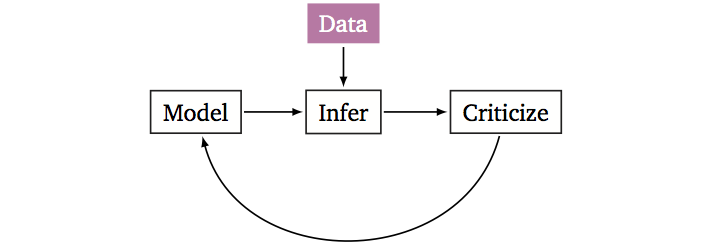
\includegraphics{images/model_infer_criticize.png}

Here's a toy example. A child flips a coin ten times, with the set of
outcomes being \texttt{{[}0,\ 1,\ 0,\ 0,\ 0,\ 0,\ 0,\ 0,\ 0,\ 1{]}},
where \texttt{0} denotes tails and \texttt{1} denotes heads. She
is interested in the probability that the coin lands heads. First,
build a model: assume the coin flips are independent and land heads with
the same probability. Second, reason about the phenomenon: use an algorithm
to infer the model given data. Third, criticize the model: analyze
whether the model captures the real-world phenomenon of coin flips. If it
doesn't, then revise the model and repeat.

This process defines the design of Edward. Four objects enable this
analysis.

\subsubsection{Data}

Data defines a set of observations. In Edward, data is represented as
TensorFlow tensors or NumPy arrays.

\begin{lstlisting}[language=Python]
x_data = np.array([0, 1, 0, 0, 0, 0, 0, 0, 0, 1])
\end{lstlisting}

Edward can also work with batch tensors for settings when the full
data does not fit in memory.

\subsubsection{Models}\label{models}

A probabilistic model is a joint distribution $p(x, z)$ of data $x$ and latent
variables $z$. In Edward, we specify it using a simple language of
random variables.

\begin{lstlisting}[language=Python]
p = Beta(a=1.0, b=1.0)
x = Bernoulli(p=tf.ones(10) * p)
\end{lstlisting}

Here, we define \texttt{p} as a scalar random variable. It is a latent
probability to a Bernoulli likelihood, and this probability is shared
across data points.

Edward also supports other languages for specifying probability models:
TensorFlow, Python, PyMC3, and Stan. More details are available in the
\href{/api/models}{model API}.

\subsubsection{Inference}\label{inference}

Given a model and data, we aim to
reason about $z$: the model's hidden structure. The
posterior distribution $p(z \mid x)$ captures our reasoning: its mean
describes our best guess of the hidden structure, and its variance
describes the uncertainty around our best guess.

Edward has many inference algorithms and makes it easy
to develop new ones.

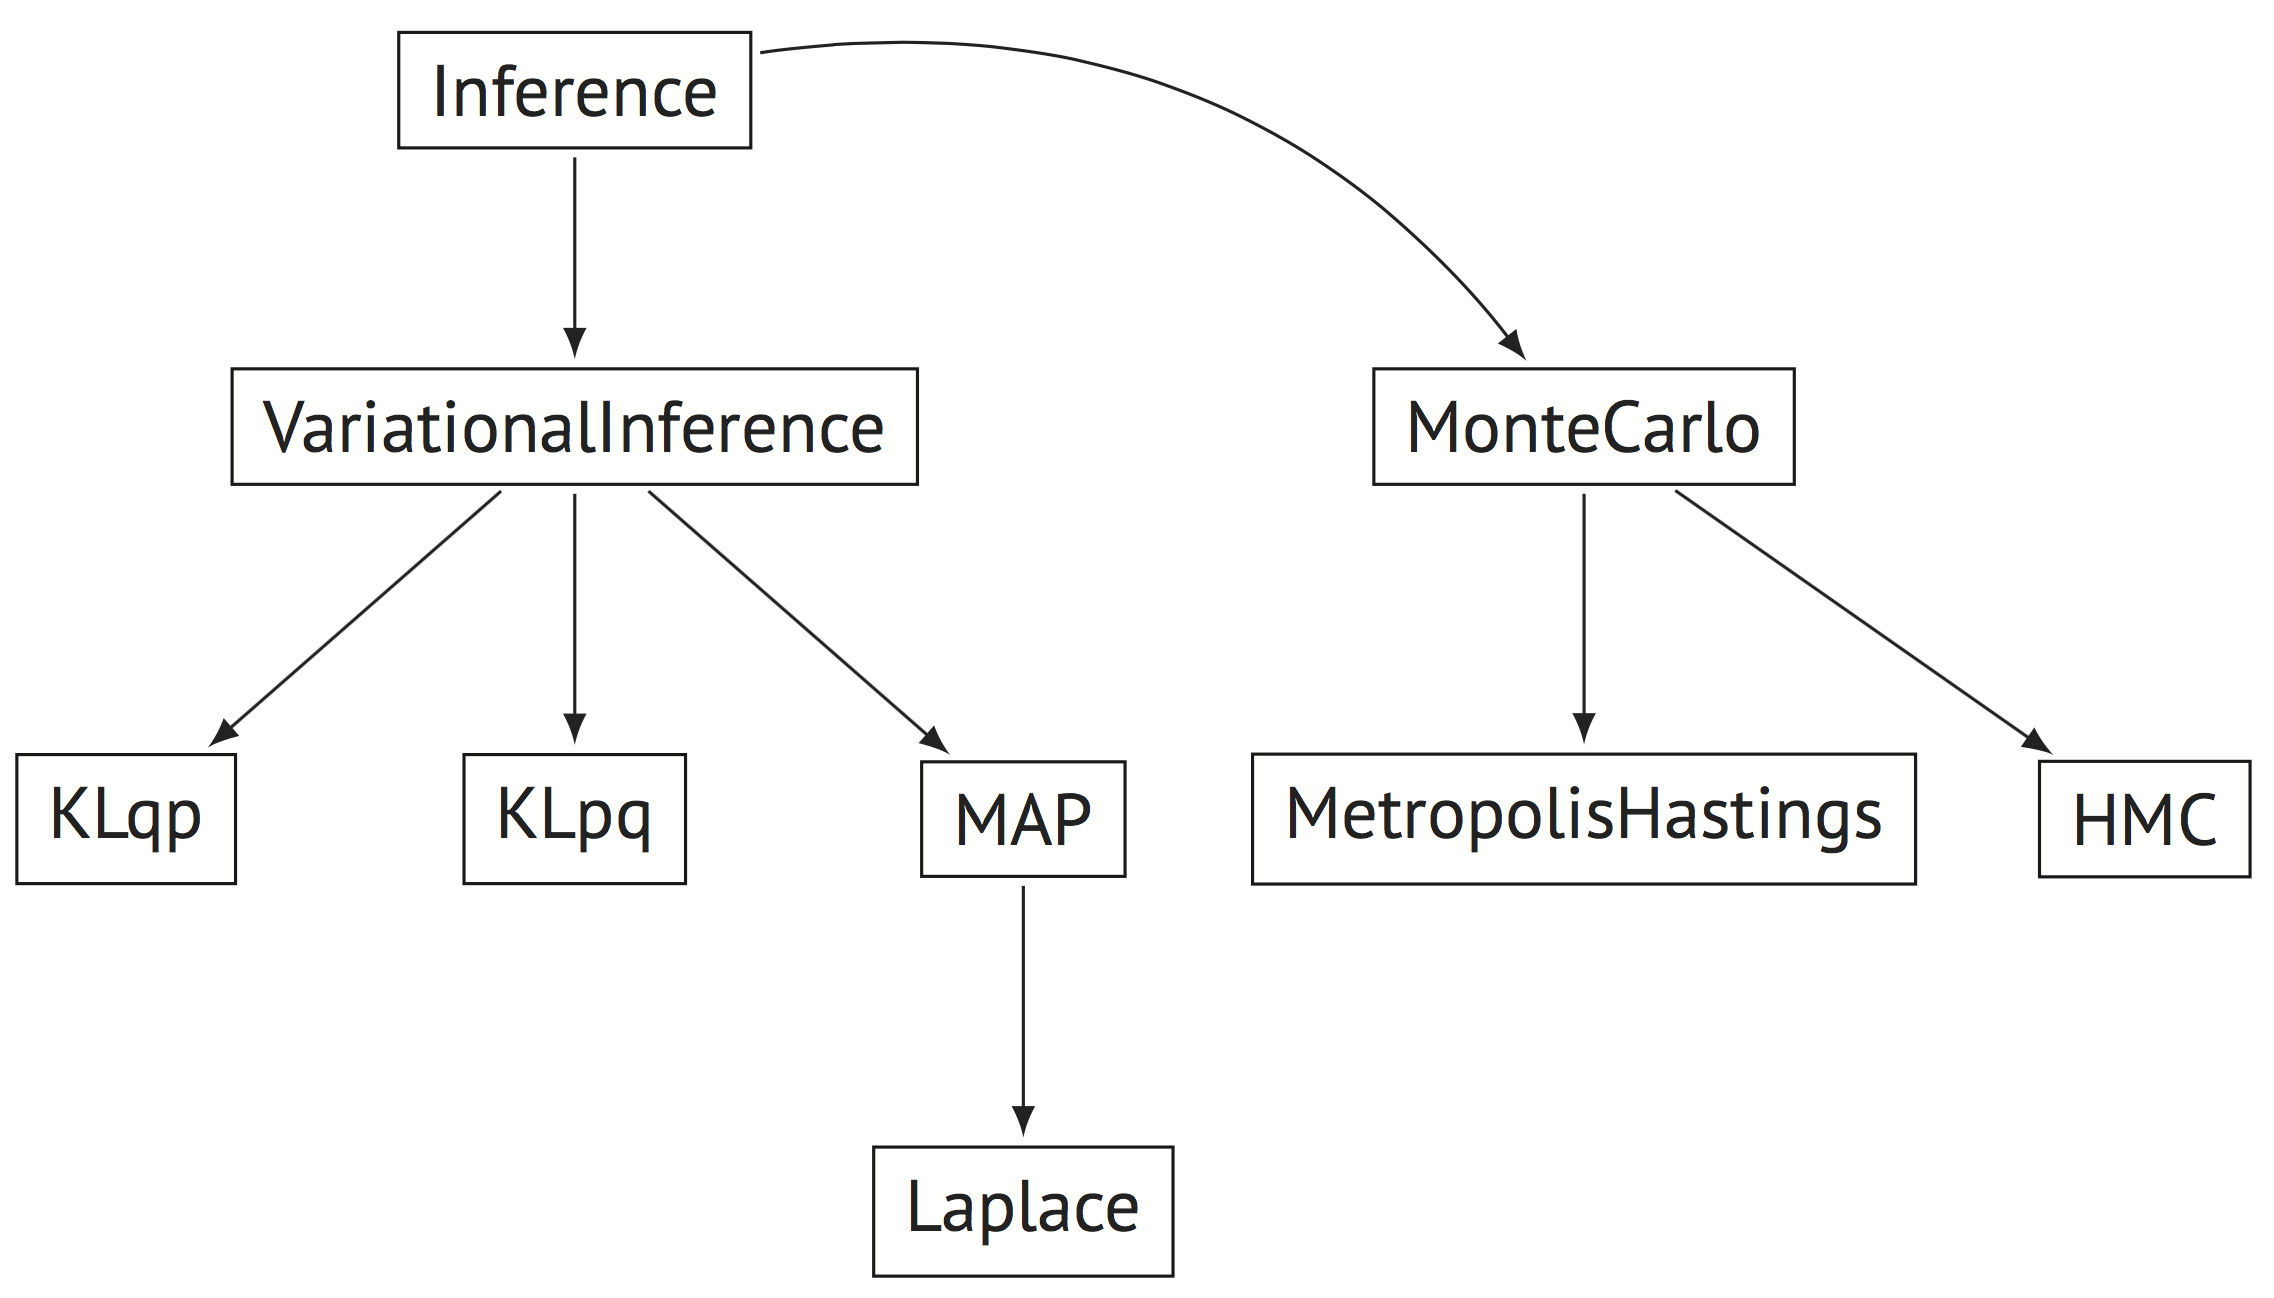
\includegraphics[width=700px]{images/inference_structure.png}
{\small\textit{Dependency graph of inference methods.
Nodes are classes in Edward and arrows represent class inheritance.}}

Edward focuses on variational inference. It views posterior inference
as positing a model of the latent variables $q(z \;;\; \lambda)$ and optimizing it to
approximate the posterior $p(z \mid x)$.

Variational models are defined using the same language of random
variables. For example, to specify a variational model (e.g.~for a
Gaussian mixture)
\begin{align*}
  q(z \;;\; \lambda)
  &=
  \text{Dirichlet}(z_\pi)
  \times
  \mathcal{N}(z_\mu)
  \times
  \text{InverseGamma}(z_\sigma)
\end{align*}
we would write
\begin{lstlisting}[language=Python]
from edward.models import Dirichlet, Normal, InverseGamma

qpi_alpha = tf.nn.softplus(tf.Variable(tf.random_normal([K])))
qmu_mu = tf.Variable(tf.random_normal([K * D]))
qmu_sigma = tf.nn.softplus(tf.Variable(tf.random_normal([K * D])))
qsigma_alpha = tf.nn.softplus(tf.Variable(tf.random_normal([K * D])))
qsigma_beta = tf.nn.softplus(tf.Variable(tf.random_normal([K * D])))

qpi = Dirichlet(alpha=qpi_alpha)
qmu = Normal(mu=qmu_mu, sigma=qmu_sigma)
qsigma = InverseGamma(alpha=qsigma_alpha, beta=qsigma_beta)
\end{lstlisting}

Each algorithm derived from \texttt{VariationalInference} minimizes a
different loss function between the variational model and the
posterior.
%They take as input a probability model \texttt{model}, a
%variational model \texttt{variational}, and data \texttt{data}.
For example, suppose we aim to minimize the Kullback-Leibler divergence
\begin{align*}
  \text{KL}(p(z \mid x) \;\|\; q(z \;;\; \lambda))
\end{align*}
Instantiate the inference class: bind each latent variable to
its corresponding variational distribution; then pass in data, which
binds each observed variable to data that we condition on. Then
run the inference.
\begin{lstlisting}[language=Python]
data = {x: x_data}
inference = ed.KLpq({pi: qpi, mu: qmu, sigma: qsigma}, data)
inference.run(n_iter=500, n_minibatch=5)
\end{lstlisting}
This runs the \texttt{KLpq} minimization algorithm for \texttt{500} iterations,
using a batch of \texttt{5} data points per iteration.

\subsubsection{Criticism}\label{criticism}

Criticizing models and their inference is a crucial step in analysis.
Following falsificationists such as Popper and Box, no model will exactly
describe the natural phenomena we seek to analyze; in other words, ``all models
are wrong''. Thus we would like to uncover where and how the model goes wrong.

Edward explores model and inference criticism using
\begin{itemize}
  \item point-based evaluations, such as mean squared error or
  classification accuracy
\end{itemize}
\begin{lstlisting}[language=Python]
ed.evaluate('mean_squared_error', data={y: y_data, x: x_data})
\end{lstlisting}
\begin{itemize}
  \item posterior predictive checks, for making probabilistic
  assessments of the model fit using discrepancy functions
\end{itemize}
\begin{lstlisting}[language=Python]
T = lambda xs, zs: tf.reduce_mean(xs[x])
ed.ppc(T, data={x: x_data})
\end{lstlisting}

See the \href{/tutorials/}{tutorials} for examples of models,
inference, and criticism in Edward.

See the \href{/api/}{API} for details of how Edward implements these
objects.

\subsubsection{References}\label{references}
